%\documentstyle[11pt,fullpage]{article}
%\setlength{\parindent}{0 in}
%\setlength{\parskip}{.1in}
%\setlength{\topmargin}{-0.5in}
%\setlength{\textheight}{8.5in}
%\begin{document}


%
% personal commentary:
%        DRAFT DRAFT DRAFT
%        - GNGUYEN
%
\chapter{Local Area Networks}
\label{chap:lan}

The characteristics of the wireless and local area networks (LAN) are
inherently different from those of point-to-point links.  A network
consisting of multiple point-to-point links cannot capture the sharing
and contention properties of a LAN.  To simulate these properties, we
created a new type of a Node, called \code{LanNode}.  The OTcl
configurations and interfaces for \code{LanNode} reside in the following
two files in the main \ns\ directory:

\begin{verbatim}
        tcl/lan/vlan.tcl
        tcl/lan/ns-ll.tcl
        tcl/lan/ns-mac.tcl
\end{verbatim}

\section{Tcl configuration}
\label{sec:lan_tcl}

The interface for creating and configuring a LAN slightly differs from
those of point-to-point link.  At the top level, the OTcl class
\code{Simulator} exports a new method called \code{make-lan}.  The
parameters to this method are similar to the method \code{duplex-link},
except that \code{make-lan} only accepts a list of nodes as a single
parameter instead of 2 parameters as in \code{duplex-link}:

\begin{verbatim}
Simulator instproc make-lan {nodes bw delay lltype ifqtype mactype chantype}
\end{verbatim}

The optional parameters to \code{make-lan} specify the type of objects
to be created for the link layer (\code{LL}), the interface queue, the
MAC layer (\code{Mac}), and the physical layer (\code{Channel}).  Below
is an example of how a new CSMA/CD (Ethernet) LAN is created.

Example:
\begin{program}
        $ns make-lan "$n1 $n2" $bw $delay LL Queue/DropTail Mac/Csma/Cd
\end{program}
creates a LAN with basic link-layer, drop-tail queue, and CSMA/CD MAC.


\section{Components of a LAN}
\label{sec:lan_components}

LanLink captures the functionality of the three lowest layers in the
network stack:

\begin{enumerate}
\item
	Link Layer (LL)
\item
	Medium Access Control (MAC) Layer
\item
	Physical (PHY) Layer
\end{enumerate}

\begin{figure}[tb]
  \centerline{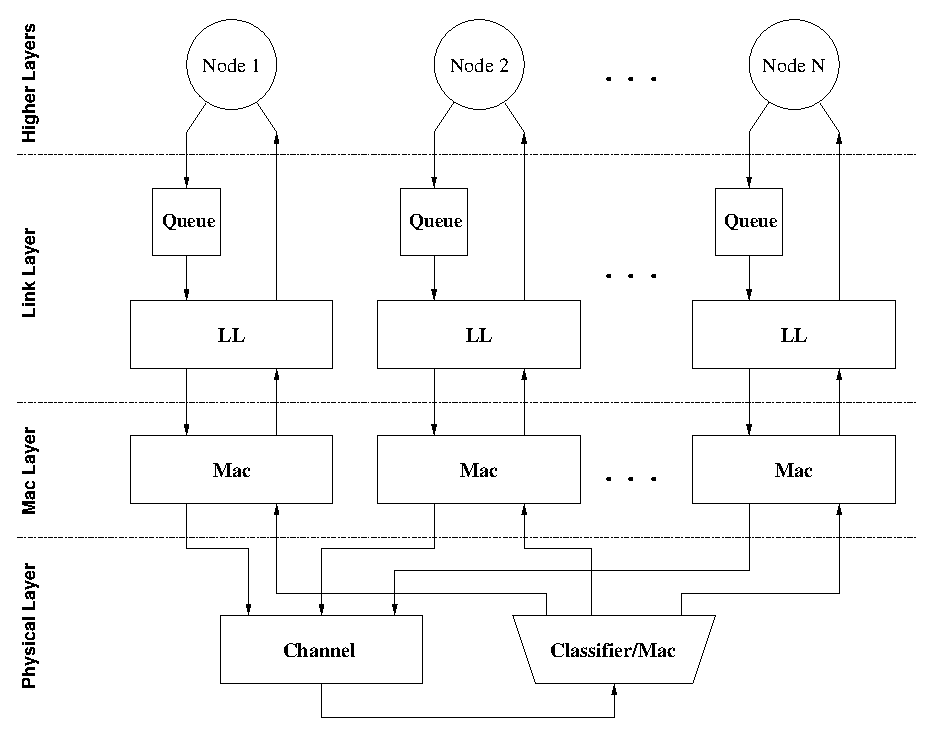
\includegraphics{lan1}}
  \caption{Connectivity within a LAN}
  \label{fig:lan-connectivity}
\end{figure}


Figure~\ref{fig:lan-connectivity} illustrates the extended network
stack that makes simulations of local area network possible in \ns.  A
packet sent down the stack flows
through the link layer (\code{Queue} and \code{LL}), the MAC layer
(\code{Mac}), and the physical layer (\code{Channel} to
\code{Classifier/Mac}).  The packet then makes its way up the stack through
the \code{Mac}, and the \code{LL}.

At the bottom of the stack, the physical layer is composed of two
simulation objects: the \code{Channel} and \code{Classifier/Mac}.  The
\code{Channel} object simulates the shared medium and supports the medium
access mechanisms of the MAC objects on the sending side of the
transmission.  On the receiving side, the \code{Classifier/Mac} is
responsible for delivering and optionally replicating packets to the
receiving MAC objects.

Depending on the type of physical layer, the MAC layer must contain a
certain set of functionalities such as: carrier sense, collision
detection, collision avoidance, etc.  Since these functionalities affect
both the sending and receiving sides, they are implemented in a single
\code{Mac} object.  For sending, the \code{Mac} object must follow a certain
medium access protocol before transmitting the packet on the channel.
For receiving, the MAC layer is responsible for delivering the packet to
the link layer.

Above the MAC layer, the link layer can potentially have many
functionalities such as queuing and link-level retransmission.  The
need of having a wide variety of link-level schemes leads to the
division of functionality into two components: \code{Queue} and
\code{LL} (link-layer).  The \code{Queue} object, simulating the
interface queue, belongs to the same \code{Queue} class that is
described in Chapter~\ref{chap:qmgmt}.  The \code{LL} object implements
a particular data link protocol, such as ARQ.  By combining both the
sending and receiving functionalities into one module, the \code{LL}
object can also support other mechanisms such as piggybacking.

\section{Channel Class}
\label{sec:channel}

The \code{Channel} class simulates the actual transmission of the packet
at the physical layer.  The basic \code{Channel} implements a shared
medium with support for contention mechanisms.  It allows the MAC to
carry out carrier sense, contention, and collision detection.  If more
than one transmissions overlaps in time, a channel raises the collision
flag.  By checking this flag, the MAC object can implement collision detection
and handling.

Since the transmission time is a function of the number of bits in the
packet and the modulation speed of each individual interface (MAC), the
\code{Channel} object only sets its busy signal for the duration
requested by the MAC object.  It also schedules the packets to be
delivered to the destination MAC objects after the transmission time
plus the propagation delay.

\subsection{Channel State}
\label{sec:channelstate}

The C++ \clsref{Channel}{../ns-2/channel.h} includes enough internal
state to schedule packet delivery and detect collisions.  It exports the
following OTcl configuration parameter:

\begin{tabularx}{\linewidth}{rX}
\code{delay\_} & propagation delay on the channel \\
\end{tabularx}

\subsection{Example: Channel and classifier of the physical layer}
\label{ex:channel}

\begin{verbatim}
        set channel_ [new Channel]
        $channel_ set delay_ 4us        # propagation delay

        set mcl_ [new Classifier/Mac]
        $channel_ target $mcl_
        $mcl_ install $mac_DA $recv_iface
                . . .
\end{verbatim}

\subsection{Channel Class in C++}
\label{sec:channelcplus}

In C++, the class Channel extends the Connector object
with several new methods to
support a variety of MAC protocols.  The class is defined as follow in
\nsf{channel.h}:

\begin{program}
   class Channel : public Connector \{
   public:
        Channel();
        void recv(Packet* p, Handler*);
        virtual int send(Packet* p, double txtime);
        virtual void contention(Packet*, Handler*);
        int hold(double txtime);
        virtual int collision() \{ return numtx_ > 1; \}
        virtual double txstop() \{ return txstop_; \}
                . . .
   \};
\end{program}

The important methods of the class \code{Channel} are:

\begin{itemize}
\item  \code{txstop()} method returns the time when the channel will become
idle, which can be used by the MAC to implement carrier sense.
\item  \code{contention()} method allows the MAC to contend for the channel
before sending a packet.  The channel then use this packet to signal the
corresponding \code{Mac} object at the end of each contention period.
\item  \code{collision()} method indicates whether a collision occurs
during the contention period.  When the \code{Channel} signal the end of
the contention period, the MAC can use the \code{collision()} method to
detect collision.
\item  \code{send()} method allows the MAC object to transmit a packet on the
channel for a specified duration of time.
\item  \code{hold()} method allows the MAC object to hold the channel for a
specified duration of time without actually transmitting any packets.
This is useful in simulating the jamming mechanism of some MAC
protocols.
\end{itemize}

\section{MacClassifier Class}
\label{sec:mac_classifier}

The \code{MacClassifier} class extends the \code{Classifier} class to
implement a simple broadcasting mechanism.  It modifies the
\code{recv()} method in the following way: since the replication of a
packet is expensive, normally a unicast packet will be classified by
the MAC destination address \code{macDA_} and delivered directly to
the MAC object with such an address.  However, if the destination
object cannot be found or if the MAC destination address is explicitly
set to the broadcast address \code{BCAST_ADDR}, the packet will be
replicated and sent to all MACs on the lan excluding the one that is
the source of the packet.  Finally, by setting the bound variable
\code{MacClassifier::bcast_} to a non--zero value, will cause
\code{MacClassifier} always to replicate packets.

\begin{program}
    class MacClassifier : public Classifier \{
    public:
        void recv(Packet*, Handler*);
    \};

    void MacClassifier::recv(Packet* p, Handler*)
    \{
        Mac* mac;
        hdr_mac* mh = hdr_mac::access(p);

        if (bcast_ || mh->macDA() == BCAST_ADDR || (mac = (Mac *)find(p)) == 0) \{
                // Replicate packets to all slots (broadcast)
                . . .
                return;
        \}
        mac->recv(p);
    \}
\end{program}


\section{MAC Class}
\label{sec:mac}

The \code{Mac} object simulates the medium access protocols that are
necessary in the shared medium environment such as the wireless and
local area networks.  Since the sending and receiving mechanisms are
tightly coupled in most types of MAC layers,
it is essential for the \code{Mac} object to be duplex.

On the sending side, the \code{Mac} object is responsible for adding the
MAC header and transmitting the packet onto the channel.  On the
receiving side, the \code{Mac} object asynchronously receives packets
from the classifier of the physical layer.  After MAC protocol
processing, it passes the data packet to the link layer.

\subsection{Mac State}
\label{sec:macstate}

The C++ \clsref{Mac}{../ns-2/mac.h} class contains enough internal state
to simulate the particular MAC protocol.  It also exports the following
OTcl configuration parameter:

\begin{tabularx}{\linewidth}{rX}
\code{bandwidth\_} & modulation rate of the MAC \\
\code{hlen\_} & additional bytes added to packet for MAC header \\
\code{label\_} & MAC address \\
\end{tabularx}

\subsection{Mac Methods}
\label{sec:macmethods}

The \clsref{Mac}{../ns-2/mac.cc} class added several Tcl methods for
configuration, in particular, linking with other simulation objects:

\begin{tabularx}{\linewidth}{rX}
\code{channel} & specify the channel for transmission \\
\code{classifier} & the classifier that deliver packets to receiving MAC \\
\code{maclist} & a link list of MAC interfaces on the same node \\
\end{tabularx}

\subsection{Mac Class in C++}
\label{sec:maccplus}

In C++, the \code{Mac} class derives from \code{Connector}.  When the
\code{recv()} method gets a packet, it identifies the direction of the
packet based on the presence of a callback handler.  If there is a
callback handler, the packet is outgoing, otherwise, it is incoming.

\begin{program}
   class Mac : public Connector \{
   public:
        Mac();
        virtual void recv(Packet* p, Handler* h);
        virtual void send(Packet* p);
        virtual void resume(Packet* p = 0);
                . . .
    \};
\end{program}

When a \code{Mac} object receives a packet via its \code{recv()} method,
it checks whether the packet is outgoing or incoming.  For an outgoing
packet, it assumes that the link-layer of the sender has obtained the
destination MAC address and filled in the \code{macDA\_} field of the
MAC header, \code{hdr_mac}.  The \code{Mac} object fills in the rest of
the MAC header with the source MAC address and the frame type.  It then
passes the packet to its \code{send()} method, which carries out the
medium access protocol.  For the basic \code{Mac} object, the
\code{send} method calls \code{txtime()} to compute the transmission
time, then invokes \code{Channel::send} to transmit the packet.  
Finally, it 
schedules itself to resume after the transmission time has elapsed.

For an incoming packet, the MAC object does its protocol processing and
passes the packet to the link-layer.

\subsection{CSMA-based MAC}

The \clsref{CsmaMac}{../ns-2/mac-csma.cc} extends the \code{Mac} class
with new methods that implements carrier sense and backoff mechanisms.
The \code{CsmaMac::send()} method detects when the channel becomes idle
using \code{Channel::txtime()}.  If the channel is busy, the MAC
schedules the next carrier sense at the moment the channel turns idle.
Once the channel is idle, the \code{CsmaMac} object initiates the
contention period with \code{Channel::contention()}.  At the end of the
contention period, the \code{endofContention()} method is invoked.  At
this time, the basic \code{CsmaMac} just transmits the packet using
\code{Channel::send}.

\begin{program}
    class CsmaMac : public Mac \{
    public:
        CsmaMac();
        void send(Packet* p);
        void resume(Packet* p = 0);
        virtual void endofContention(Packet* p);
        virtual void backoff(Handler* h, Packet* p, double delay=0);
                . . .
    \};

    class CsmaCdMac : public CsmaMac \{
    public:
        CsmaCdMac();
        void endofContention(Packet*);
    \};

    class CsmaCaMac : public CsmaMac \{
    public:
        CsmaCaMac();
        virtual void send(Packet*);
    \};
\end{program}

The \code{CsmaCdMac} extends \code{CsmaMac} to carry out collision
detection procedure of the CSMA/CD (Ethernet) protocol.  When the
channel signals the end of contention period, the \code{endofContention}
method checks for collision using the \code{Channel::collision()}
method.  If there is a collision, the MAC invokes its \code{backoff}
method to schedule the next carrier sense to retransmit the packet.

The \code{CsmaCaMac} extends the \code{send} method of \code{CsmaMac} to
carry out the collision avoidance (CSMA/CA) procedure.  Instead of
transmitting immediately when the channel is idle, the \code{CsmaCaMac}
object backs off a random number of slots, then transmits if the channel
remains idle until the end of the backoff period.

\section{LL (link-layer) Class}
\label{sec:linklayer}

The link-layer object is responsible for simulating the data link
protocols.  Many protocols can be implemented within this layer such
as packet fragmentation and reassembly, and reliable link protocol. 

Another important function of the link layer is setting the MAC
destination address in the MAC header of the packet.  In the current
implementation this task involves two separate issues: finding the
next--hop--node's IP address (routing) and resolving this IP address
into the correct MAC address (ARP).  For simplicity, the default
mapping between MAC and IP addresses is one--to--one, which means that
IP addresses are re--used at the MAC layer.

\subsection{LL Class in C++}
\label{sec:llcplus}

The C++ class \code{LL} derives from the \code{LinkDelay} class.  Since
it is a duplex object, it keeps a separate pointer for the send target,
\code{sendtarget}, and the receive target, \code{recvtarget}.  It also
defines the methods \code{recvfrom()} and \code{sendto()} to handle the
incoming and outgoing packets respectively.

\begin{program}
   class LL : public LinkDelay \{
   public:
   	   LL();
   	   virtual void recv(Packet* p, Handler* h);
   	   virtual Packet* sendto(Packet* p, Handler* h = 0);
   	   virtual Packet* recvfrom(Packet* p);
   
   	   inline int seqno() { return seqno_; }
   	   inline int ackno() { return ackno_; }
   	   inline int macDA() { return macDA_; }
   	   inline Queue *ifq() { return ifq_; }
   	   inline NsObject* sendtarget() { return sendtarget_; }
   	   inline NsObject* recvtarget() { return recvtarget_; }
   
   protected:
   	   int command(int argc, const char*const* argv);
   	   void handle(Event* e) { recv((Packet*)e, 0); }
   	   inline virtual int arp (int ip_addr) { return ip_addr; } 
   	   int seqno_;			// link-layer sequence number
   	   int ackno_;			// ACK received so far
   	   int macDA_;			// destination MAC address
   	   Queue* ifq_;			// interface queue
   	   NsObject* sendtarget_;		// for outgoing packet 
   	   NsObject* recvtarget_;		// for incoming packet
   
   	   LanRouter* lanrouter_; // for lookups of the next hop
   \};
\end{program}

\subsection{Example: Link Layer configuration}
\label{ex:linklayer}

\begin{program}
    set ll_  [new LL]
    set ifq_ [new Queue/DropTail]
    $ll_ lanrouter  [new LanRouter $ns $lan] # LanRouter is one object
                                             # per LAN
    $ll_ set delay_ $delay        # link-level overhead
    $ll_ set bandwidth_ $bw       # bandwidth
    $ll_ sendtarget $mac          # interface queue at the sender side
    $ll_ recvtarget $iif          # input interface of the receiver
             . . .
\end{program}

\section{\code{LanRouter} class}
By default, there is just one \code{LanRouter} object per LAN, which
is created when a new \code{LanNode} is initialized.  For every node
on the LAN, the link layer object (\code{LL}) has a pointer to the
\code{LanRouter}, so it is able to find the next hop for the packet
that is sent on the LAN:
\begin{program}
Packet* LL::sendto(Packet* p, Handler* h)
\{        
        int nh = (lanrouter_) ? lanrouter_->next_hop(p) : -1;
        . . .
\}
\end{program}
\code{LanRouter} is able to find the next hop by querying the current
\code{RouteLogic}:
\begin{program}
int LanRouter::next_hop(Packet *p) \{
        int next_hopIP;
        if (enableHrouting_) \{
                routelogic_->lookup_hier(lanaddr_, adst, next_hopIP);
        \} else \{
                routelogic_->lookup_flat(lanaddr_, adst, next_hopIP);
        \}
\end{program}
One limitation of this is that \code{RouteLogic} may not be aware of
dynamic changes to the routing.  But it is always possible to derive a
new class from \code{LanRouter} so that to re--define its
\code{next_hop} method to handle dynamic changes appopriately.

\section{Other Components}
\label{sec:lan_others}

In addition to the C++ components described above, simulating local area
networks also requires a number of existing components in \ns\ such as
\code{Classifier}, \code{Queue}, and \code{Trace},
\code{networkinterface}, etc.  Configuring these
objects requires knowledge of what the user wants to simulate.  The
default configuration is implemented in the two Tcl files mentioned at
the beginning of this chapter.  To obtain more realistic simulations
of wireless networks, one can use the \code{ErrorModel} described in
Chapter~\ref{chap:error_model}.

\section{LANs and \ns\ routing}
\label{sec:lan_ns-routing}

When a LAN is created using either \code{make-lan} or \code{newLan}, a
``\textit{virtual LAN node}'' \code{LanNode} is created.
\code{LanNode} keeps together all shared objects on the LAN:
\code{Channel}, \code{Classifier/Mac}, and \code{LanRouter}.  Then for
each node on the LAN, a \code{LanIface} object is created.
\code{LanIface} contains all other objects that are needed on the
per--node basis: a \code{Queue}, a link layer (\code{LL}),
\code{Mac}, etc.  It should be emphasized that \code{LanNode} is a
node only for routing algorithms:  \code{Node} and \code{LanNode} have
very little in common.  One of few things that they share is an
identifier taken from the \code{Node} ID--space.  If
\textit{hierarchical routing} is used, \code{LanNode} \textit{has to be
assigned a hierarchical address} just like any other node.  From the
point of view of \ns\ (static) routing, \code{LanNode} is just another
node connected to every node on the LAN.
\begin{figure}[hbt]
	\centerline{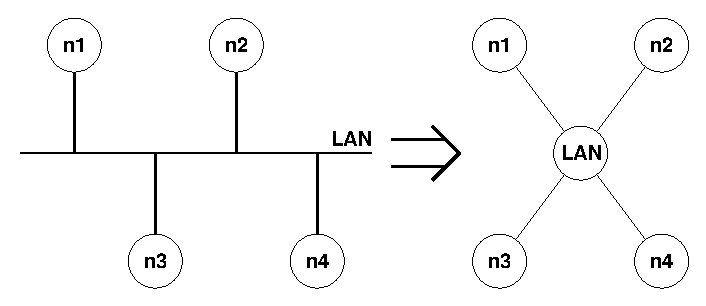
\includegraphics{lan2}}
  	\caption{Actual LAN configuration (left) and as seen by
  	\ns\ routing (right)}
  	\label{fig:lan-routing1}
\end{figure}
Links connecting the \code{LanNode} with the nodes on the LAN are also
``virtual'' (\code{Vlink}).  The default routing cost of such a link
is $1/2$, so the cost of traversing two \code{Vlink}s
(e.g. \textbf{n1 $\rightarrow$ LAN $\rightarrow$ n2}) is counted as just one
hop.  

Most important method of \code{Vlink} is the one that gives the head
of the link:
\begin{program}
Vlink instproc head \{\} \{
    $self instvar lan_ dst_ src_
    if \{$src_ == [$lan_ set id_]\} \{
        # if this is a link FROM the lan vnode, 
        # it doesn't matter what we return, because
        # it's only used by $lan add-route (empty)
        return ""
    \} else \{
        # if this is a link TO the lan vnode, 
        # return the entry to the lanIface object
        set src_lif [$lan_ set lanIface_($src_)]
        return [$src_lif entry]
    \}
\}
\end{program}
This method is used by static (default) routing to install correct
routes at a  node (see \code{Simulator} methods \\ \code{compute-flat-routes} and
\code{compute-hier-routes} in \code{tcl/lib/ns-route.tcl}, as well
as \code{Node} methods \code{add-route} and \code{add-hroute} in
\code{tcl/lib/ns-node.tcl}).  

From the code fragment above it can be seen that it returns LAN
interface of the node as a head of the link to be installed in the
appropriate classifier. 

Thus, \code{Vlink} \textit{does not impose any delay on the packet}
and serves the only purpose to install LAN interfaces instead of
normal links at nodes' classifiers.  

Note, that this design allows to have nodes connected by parallel
LANs, while in the current implementation it is impossible to have
nodes connected by parallel simple links and use them both (the array
\code{Simulator instvar link_} holds the link object for each
connected pair of source and destination, and it can be only one
object per source/destination pair).

\section{Commands at a glance}
\label{sec:lancommand}

\begin{program}
$ns_ make-lan  <nodelist> <bw> <delay> <LL> <ifq> <MAC> <channel> <phy>
\end{program}
Creates a lan from a set of nodes given by <nodelist>. Bandwidth, delay characteristics
along with the link-layer, Interface queue, Mac layer and channel type for the
lan also needs to be defined. Default values used are as follows:
<LL> .. LL
<ifq>.. Queue/DropTail
<MAC>.. Mac
<channel>.. Channel
<phy>.. Phy/WiredPhy


\begin{program}
$ns_ newLan <nodelist> <BW> <delay> <args>
\end{program}
This command creates a lan similar to make-lan described above. But this
command can be used for finer control whereas make-lan is a more convinient and
easier command. For example newLan maybe used to create a lan with hierarchical
addresses. See \ns/tcl/ex/{vlantest-hier.tcl, vlantest-mcst.tcl, lantest.tcl,
mac-test.tcl} for usage of newLan. The possible argument types that can be passed
are LL, ifq, MAC, channel, phy and address.

\begin{program}
$lannode cost <c>
\end{program}
This assigns a cost of c/2 to each of the (uni-directional) links in the lan.

\begin{program}
$lannode cost?
\end{program}
Returns the cost of (bi-directional) links in the lan, i.e c.


Internal procedures :

\begin{program}
$lannode addNode <nodes> <bw> <delay> <LL> <ifq> <MAC> <phy>
\end{program}
Lan is implemented as a virtual node. The LanNode mimics a real node and uses
an address (id) from node's address space.
This command adds a list of <nodes> to the lan represented by lannode.
The bandwidth, delay and network characteristics of nodes are given by
the above arguments. This is an internal command used by make-lan and newLan.

\begin{program}
$lannode id
\end{program}
Returns the virtual node's id.

\begin{program}
$lannode node-addr
\end{program}
Returns virtual nodes's address.

\begin{program}
$lannode dump-namconfig
\end{program}
This command creates a given lan layout in nam. This function may be changed
to redefine the lan layout in a different way.

\begin{program}
$lannode is-lan?
\end{program}
This command always returns 1, since the node here is a virtual node
representing a lan. The corresponding command for node \code{$node is-lan?}
always returns a 0.


%\end{document}
\endinput



